%harihiom
\documentclass{llncs}

\usepackage[english]{babel}
%\usepackage[utf8]{inputenc}
%\usepackage{amsmath}
\usepackage{graphicx}
\usepackage{float}
%\usepackage{wrapfig}
%\usepackage{titlepic}
%\usepackage[colorinlistoftodos]{todonotes}
\usepackage{graphicx,epstopdf}
\usepackage{amsmath,amssymb,amsfonts,subfigure}
\usepackage{comment}
\usepackage{algorithm}
\usepackage{algpseudocode}
\usepackage{pifont}
\usepackage[normalem]{ulem}
\usepackage[english]{babel}
\usepackage[utf8x]{inputenc}
\usepackage{graphicx}
\usepackage{calc}
\usepackage{graphicx}
\usepackage{subfigure}
\usepackage{gensymb}
\usepackage{natbib}
\usepackage{url}
\usepackage[utf8x]{inputenc}
\usepackage{amsmath}
\usepackage{graphicx}
\graphicspath{{images/}}
\usepackage{parskip}
\usepackage{fancyhdr}
\usepackage{vmargin}
\usepackage{algorithm}
\linespread{1}
\usepackage{color}
\usepackage{cite}
\usepackage{amsmath,amssymb}
\newtheorem{claim1}{Claim}
\usepackage{algpseudocode}% http://ctan.org/pkg/algorithmicx
\usepackage[compatibility=false]{caption}% http://ctan.org/pkg/caption
\setmarginsrb{3 cm}{2.5 cm}{3 cm}{2.5 cm}{1 cm}{1.5 cm}{1 cm}{1.5 cm}

%\newtheorem{theorem}{Theorem}
%\newtheorem{lemma}{Lemma}

\title{Lecture - 3}
\author{Friday, 29 July 2016 (16:15 - 17:05)}
\institute{Puzzles : Cryptanalysis of Vigenere Cipher}

\begin{document}
\maketitle
\vspace{5mm}
The main aim of this lecture is to understand the cryptanalysis of the Vigenere cipher. But before that, we will get a hint of the previous basic cryptographic techniques as well. 

\section{Caesar Cipher}
\textbf{Plain Text}:\hspace{1mm} T H I S I S A S E C R E T\\

The value of key $k$ is from $1$ to $26$. We shift each alphabet of the plain text by $k$ places. \\
If $k=2$,

\begin{table}[h]
\begin{center}
\begin{tabular}{ |c|c|c|c|c|c|c|c|c|c|c|c|c|c|c| }
\hline
\textbf{Plain Text} & T & H & I & S & I & S & A & S & E & C & R & E & T \\
\hline
\textbf{Cipher Text} & V & J & K & U & K & U & C & U & G & E & T & G & V \\
\hline
\end{tabular}\\
\vspace{2mm}
\caption{Caesar Cipher}
\label{caesar}
\end{center}
\end{table}



\textbf{Cryptanalysis\footnote{Cryptanalysis is the technique of deciphering(decoding the encrypted text back to the plain text) without knowing the key $k$)}:}
We try each of the $26$ possible combinations of $k$, and see which of these $26$ decodings make sense. 

\section{Substitution Cipher}
In this ciphering scheme, we substitute the alphabets present in the plain text by the alphabets of our choice. For example : `A' can be replaced by `$\aleph$', `B' can be replaced by `$\prime$' and so on. 
An example is shown in the Table \ref{sub}.

\begin{table}[h]
\begin{center}
\begin{tabular}{ |c|c|c|c|c|c|c|c|c|c|c|c|c|c|c| }
\hline
\textbf{Plain Text} & T & H & I & S & I & S & A & S & E & C & R & E & T \\
\hline
\textbf{Cipher Text} & $\alpha$ & $\beta$ & $\gamma$ & $\delta$ & $\gamma$ & $\delta$ & $\aleph$ & $\delta$ & $\pi$ & $\Xi$ & $\Psi$ & $\pi$ & $\alpha$ \\
\hline
\end{tabular}\\
\vspace{2mm}
\caption{Substitution Cipher}
\label{sub}
\end{center}
\end{table}

So, the key here will be a series of 26 symbols which will substitute one of the 26 alphabets of English. This seems to be a better technique as compared to the Caesar Cipher. 

\subsection{Cryptanalysis}
If we take a volume of the English text and look at the volume of different alphabets, we get a distribution. In other words, all the English alphabets are not used at the same frequency, for example- `Z' is used quite less frequently as `E'. 
\begin{itemize}
\item `A' tend to appear $8.16 \%$ of the times. 
\item `B' tend to appear $1.49 \%$ of the times. 
\item `C' tend to appear $2.78 \%$ of the times. 
\item `D' tend to appear $4.5 \%$ of the times. 
\item `E' tend to appear $12.7 \%$ of the times. 
\item `T' tend to appear $9.056 \%$ of the times. 
\item `Z' tend to appear $0.074 \%$ of the times. 
\end{itemize}

The alphabets can be arranges as following in the ascending order of their frequency distribution. \\
E, T, A, O, I, N, S, H, R, D, L, C, U, M, W, F, G, Y, P, B, V, K, J, X, Q, Z\\

In the cryptanalysis, we look at the maximum occurring letter and assign a `E' to it. The second frequent letter is assigned `T' and so on, the least frequent letter is assigned `Z'.

\section{Vigenere Cipher} 
Vigenere Cipher was first described in the year 1553. Till 1854(for like 200 years), nobody was able to break this cipher and it was considered to be exceptionally strong. It was in 1854, when Charles Babbage broke this cipher. 

\subsection{How does Vigenere Cipher Work}

The Figure \ref{vigenere} explains the working of vigenere cipher.

\begin{figure}[h]
\centering
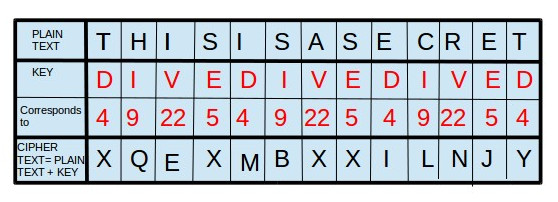
\includegraphics[width=0.9\textwidth]{vigenere.jpg}
\label{vigenere}
\caption{Working of Vigenere cipher}
\end{figure}

It can be seen as a combination of Caesar cipher and substitution cipher. Every alphabet of the plain text is shifted by a different number depending upon the letter of the key corresponding to that place. So, at some places, the same alphabet can be shifted by 5, rather at some places, it can be shifted by 22 and so on. Hence, the final result does not follow the frequency distribution of the English alphabets. 

\subsection{Cryptanalysis}

\textbf{Observe that} if the key length is known in the Vigenere cipher, then the cryptanalysis is straightforward. \\

\textbf{{\large How:-}}Assume that the length of the key is $l$, then we know that the alphabets at the locations $i$, $i+l$, $i+2l$, .... are shifted by the same number, since they all correspond to the same key letter. Example- In Figure \ref{vigenere}, the size of the key is 4. Hence, the alphabets at locations 1, 5, 9 and 13 are all shifted by the same number(4 corresponding to `D'). Similarly, alphabets at locations 2, 6 and 10 are shifted by same number(9 corresponding to `I') and so on. \\

So, if take the set of alphabets of cipher text at the locations $i$, $i+l$, $i+2l$, ...., they form an instance of the substitution cipher itself, where an alphabet is substituted by the same symbol or the same another alphabet since they are shifted by an equal number. If we look at the frequency distribution of this subset, it should follow the English frequency distribution. So, now we do the same thing as in the substitution cipher. Replace the maximum occurring alphabet in this subset of cipher text by `E', second maximum occurring by `T' and so on. \\

\[
 \boxed{\textbf{The\ question\ which\ still\ remains\ is\ how\ to\ find\ the\ key\ length?}}
 \]
 
\textbf{{\large Finding Key Length:-}} Let $S$ be a string of length $N$, where $N$ is a very large number, say $N = 10^6$. \\

$S = s_1\ s_2\ s_3\ ...\ s_{10^6-1}\ s_{10^6}$\\

Let $L$ be the number of letters in a language, for example, $L=26$ for English. \\

If we pick two letters from $S$, probability that they are same = \textbf{?}. \\

Number of ways in which two distinct letters can be picked from $S$ = $N \times (N-1)$ (considering ordered pair). Assume a letter $s_i$ occurs $p_i$ number of times in $S$. \\

Then probability that the picked letters $s_i$ and $s_j$ are same = $\sum_{i=1}^L \frac{(p_i) \times (p_i - 1)}{ N \times (N-1)}$ \\

We take the summation from $1$ to $L$ because the picked letter can be any letter from the set of letters of the language. \\

$\sum_{i=1}^L \frac{(p_i) \times (p_i - 1)}{ N \times (N-1)}$\\

= $ \frac{1}{ N \times (N-1)}\sum_{i=1}^L (p_i) \times (p_i - 1)$\\

= $ \frac{1}{ N \times (N-1)}\sum_{i=1}^L (f_i.N) \times (f_i.N\ - 1)$\\

= $ \frac{1}{N-1}\sum_{i=1}^L (f_i) \times (f_i\ - 1)$\\

= $\sum_{i=1}^L f_i \times f_i$		\hspace{5mm} since $N$ is a very large number\\

= $\sum_{i=1}^L {f_i}^2$\\

= $6.8 \times {10}^{-2}$, for English language\\

\textbf{How does this result help us?}: If the given text was to be random, instead of the massive text from English(or some other language), then all the $f_i$s would be the same. In that case\\	

$\sum_{i=1}^L {f_i}^2$\\

=$\sum_{i=1}^{26} {\frac{1}{26}}^2$\\

= $3.8 \times {10}^{-2}$  \\

This difference in both the cases helps us in finding the key length. Let us see how. \\

Given a cipher text, rotate the text by 1 letter and look at the number of collisions as shown in the Figure \ref{vigc}. Please note that the figure is used just to explain the rotation and counting concept. 

\begin{figure}[h]
\centering
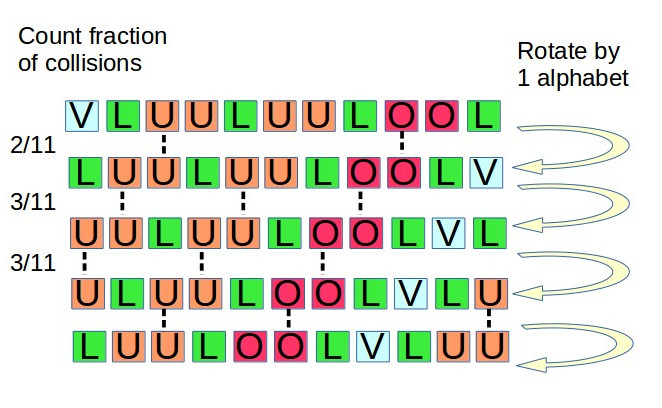
\includegraphics[width=0.9\textwidth]{vig_c.jpg}
\label{vigc}
\caption{Finding key length $l$ in vigenere cipher}
\end{figure}

As shown in the figure, we keep rotating the cipher text and look at the fraction of collisions. The mega result is : \\

\textbf{\textit{The fraction of collisions mostly is 3.8 \%, but as soon as the number of rotations becomes equal to the key length $l$, the fraction of collisions increases to 6.8\%.}} 
\end{document}